% ============================================================
% Collateral Damage in Graph-based Memory Forgetting:
% Quantification, Exploitation, and Defense
% SCALE Workshop @ ICML 2026 (7-page version)
% ============================================================
\documentclass{article}

\usepackage{microtype}
\usepackage{graphicx}
\usepackage{subcaption}
\usepackage{booktabs}
\usepackage{hyperref}

\newcommand{\theHalgorithm}{\arabic{algorithm}}

% Double-blind review version
\usepackage{icml2026}

\usepackage{amsmath,amssymb}
\usepackage[capitalize,noabbrev]{cleveref}
\usepackage{multirow}
\usepackage{algorithm}
\usepackage{algorithmic}
\usepackage{xcolor}

% --- Custom Commands ---
\newcommand{\attraware}{\textsc{Attr-Aware}}
\newcommand{\bfsprop}{\textsc{BFS}}
\newcommand{\finding}[1]{\vspace{2pt}\noindent\textbf{Finding #1.}~}

\icmltitlerunning{Collateral Damage in Graph-based Memory Forgetting}

\begin{document}

\twocolumn[
  \icmltitle{Collateral Damage in Graph-based Memory Forgetting:\\
  Quantification, Exploitation, and Defense}

  \icmlaffiliation{anon}{Anonymous Institution}

  \begin{icmlauthorlist}
    \icmlauthor{Anonymous}{anon}
  \end{icmlauthorlist}

  \icmlcorrespondingauthor{Anonymous}{anonymous@example.com}

  \icmlkeywords{AI Agent Memory, Graph Propagation, Selective Forgetting, Adversarial Attacks}

  \vskip 0.3in
]
\printAffiliationsAndNotice{}

% ============================================================
\begin{abstract}
Agent memory systems increasingly use entity graphs for retrieval and consolidation, but invalidation is handled at the level of individual facts---leaving dependent facts silently stale.
Propagating invalidation through graph edges is a natural way to maintain consistency, yet \textbf{structural co-occurrence does not imply dependency}.
We implement and evaluate BFS invalidation propagation over co-occurrence graphs derived from MemoryAgentBench to stress-test this design choice.
Across 6K--64K turns, BFS propagation reduces stale retention but damages 69--79\% of valid memories. It also degrades cross-task retrieval F1 by $10.1$pp.
Hub-targeted invalidations amplify this failure: five injected facts degrade 57.3\% of valid memories under white-box access.
To mitigate over-propagation, we propose \textbf{\attraware{} Selective Propagation}, an attribute-keyed directional filter that limits cascades to plausible dependency paths. It requires no LLM calls during propagation and achieves 78--100\% defense effectiveness relative to unfiltered BFS, demonstrating that lightweight mitigation is feasible.
Our results suggest that graph-based memory forgetting should incorporate dependency-aware propagation; the optimal filtering strategy remains an open problem.
\end{abstract}

% ============================================================
\section{Introduction}
\label{sec:intro}

AI agents with persistent memory are moving from prototypes to production.
Mem0~\citep{mem0_2024} and other memory-augmented agent frameworks have proliferated across open-source and proprietary ecosystems~\citep{graph_agent_memory_survey_2026}.
These systems increasingly maintain entity graphs to organize stored facts~\citep{mem0_2024, magma_2026, zep_2025}.

As memory scales to tens of thousands of facts, maintaining consistency becomes critical---yet multi-hop conflict resolution accuracy remains below 6\% on standard benchmarks~\citep{memoryagentbench_2026}.
The gap is structural: current systems handle invalidation \textit{individually}, leaving dependent facts silently stale.
This creates concrete pressure toward propagation.
Anecdotal reports from production deployments suggest that per-fact-only invalidation leads to accumulating inconsistencies over time.\footnote{Mem0 GitHub Issues \#4573, \#4863, \#3841 (2025) describe stale entity links and contradictory facts as recurring community complaints.}
Graph-based propagation---cascading updates through entity connections---is the natural next step, and the implementation distance is short.
Zep~\citep{zep_2025} maintains temporal validity windows on graph edges; MAGMA~\citep{magma_2026} constructs explicit causal sub-graphs; Mem0~\citep{mem0_2024} already traverses entity graphs during conflict detection.
Adding weight updates to this existing traversal requires minimal code changes, creating strong pressure toward adoption.
Each system implements prerequisites for propagation without taking the final step.

We implement this step and reveal a fundamental tension.
Entity co-occurrence graphs link facts that share entities, but sharing an entity does not imply causal dependency.
``The president of Russia'' connects diplomatic facts and unrelated economic facts identically.
Co-occurrence is not an artifact of naive graph construction: even typed-relation graphs contain co-occurrence as an unavoidable substructure whenever multiple facts reference the same entity.
BFS propagation treats all such connections identically, cascading invalidation through semantically meaningless edges.

This distinction---well-understood in transportation network resilience, where directional failure models separate correlated from causally dependent links~\citep{chen_network_2007}---has not been applied to AI memory systems.
We contribute:

\begin{enumerate}
  \item \textbf{Failure formulation}: We formalize invalidation propagation as a \textit{retention-forgetting trade-off} in graph-based agent memory: insufficient propagation leaves stale facts, while raw co-occurrence propagation damages valid memories (\cref{sec:tradeoff}).

  \item \textbf{Controlled quantification}: On MemoryAgentBench-derived co-occurrence graphs, naive BFS propagation damages 69--79\% of valid memories across 6K--64K scales and degrades unrelated retrieval F1 by $10.1$pp (\cref{sec:c1}).

  \item \textbf{Hub amplification analysis}: High-degree entities amplify invalidation damage under gray-box and white-box access, while our random black-box baseline fails entirely (\cref{sec:c3}).

  \item \textbf{Mitigation feasibility}: \attraware{} propagation, a hyperparameter-free attribute-keyed filter, demonstrates that lightweight mitigation is achievable---reducing collateral damage by 78--100\% relative to unfiltered BFS without LLM calls (\cref{sec:c4}). Tuned threshold methods can match or exceed this at scale, underscoring that optimal filtering remains open.
\end{enumerate}

\noindent As a proactive safety study, we characterize failure modes of a plausible design choice \textit{before} it reaches production---providing quantified evidence that systems adopting co-occurrence graphs for memory should incorporate dependency-aware propagation from the outset.


% ============================================================
\section{Background}
\label{sec:background}

\paragraph{Graph-augmented memory systems.}
Modern AI memory systems differ in how they encode entity relationships.
\Cref{tab:systems} summarizes existing architectures along the dimension most relevant to propagation: edge semantics and invalidation strategy.
In their published descriptions, graphs serve \textit{retrieval} and consolidation but none specifies a general-purpose \textit{invalidation propagation} mechanism over entity co-occurrence edges.

\begin{table}[htbp]
\centering
\footnotesize
\begin{tabular}{llll}
\toprule
\textbf{System} & \textbf{Graph} & \textbf{Edges} & \textbf{Invalidation} \\
\midrule
Mem0$^g$ & KG & Typed & Per-fact \\
Zep & Temporal KG & Bi-temporal & Per-edge \\
MAGMA & 4 sub-graphs & Causal+Entity & Per-graph \\
A-Mem & Linked notes & Associative & Per-note \\
\bottomrule
\end{tabular}
\caption{Graph-augmented memory systems~\citep{mem0_2024, zep_2025, magma_2026, amem_2025}. $^g$graph-enabled mode. We found no explicit invalidation propagation in their published descriptions.}
\label{tab:systems}
\end{table}

\paragraph{The forgetting gap.}
MemoryAgentBench~\citep{memoryagentbench_2026} evaluates multi-hop conflict resolution where systems must update or discard outdated facts under contradictory evidence.
No tested system exceeds 6\% accuracy.
MemoryArena~\citep{memoryarena_2026} shows agents drop to 40--60\% on session-interdependent tasks.
The failure mode is consistent: systems cannot reason about \textit{dependencies between facts}.

\paragraph{Belief revision perspective.}
Kumiho~\citep{kumiho_2026} formalizes this problem through AGM belief revision~\citep{agm_1985}: typed dependency edges (e.g., \texttt{Depends\_On}, \texttt{Derived\_From}) ensure that only causally related beliefs are affected during revision.
This provides axiomatic guarantees---but requires typed edges at graph construction time, which Mem0, Zep, and MAGMA do not currently provide.
Our work addresses the complementary question: \textit{what happens when propagation is attempted on existing untyped co-occurrence graphs?}

\paragraph{Memory as an attack surface.}
MINJA~\citep{minja_2025} achieves 98\% injection success via query-only interaction; AgentPoison~\citep{agentpoison_2024} poisons 80\%+ of agent decisions by modifying $<$0.1\% of stored entries.
MITRE ATLAS designates memory manipulation as technique AML.T0080~\citep{mitre_atlas_2023}.
These attacks inject malicious \textit{content}; our work reveals a structurally distinct threat where the system's own \textit{maintenance mechanism} becomes the attack vector.

\paragraph{Structural vulnerability from graph topology.}
The content-injection attacks above exploit \textit{what} is stored; a complementary question is whether the graph \textit{structure itself} creates vulnerability.
Networks with heavy-tailed degree distributions are robust to random failures but catastrophically fragile to targeted hub removal~\citep{albert_attack_2000, cohen_percolation_2000}.
Transportation network resilience provides a structural analogy: directional failure models separate correlated from causally dependent links~\citep{chen_network_2007}, though the dynamics differ between physical and information networks.
We test whether memory co-occurrence graphs exhibit this topology and whether hub-targeted operations produce the predicted damage.


% ============================================================
\section{The Propagation Trade-off}
\label{sec:tradeoff}

Before analyzing failure modes, we establish \textit{why} propagation matters.
We design 10 fact-change scenarios (personnel changes, schedule updates) with 5 causally related and 15 unrelated memories each.
For instance, updating ``the CEO of Acme is Alice'' to ``the CEO of Acme is Bob'' should invalidate ``Alice approves Acme milestones'' (dependent) but not ``Acme was founded in 2010'' (co-occurring but independent).

\begin{table}[htbp]
\centering
\footnotesize
\begin{tabular}{lrrr}
\toprule
\textbf{Mode} & \textbf{Forget Acc.} & \textbf{Collateral} & \textbf{Stale@worst} \\
\midrule
No-Propagation & 84.0\% & 0.0\% & 40\% \\
\bfsprop{} & 96.0\% & 47.5\% & 0\% \\
\attraware{} & 94.0\% & 25.0\% & 8\% \\
\bottomrule
\end{tabular}
\caption{Forgetting benefit vs.\ collateral cost (10 controlled scenarios).
No-Propagation leaves 16\% stale (worst 40\%).
BFS achieves highest accuracy but damages 47.5\% of unrelated memories.
\attraware{} reduces collateral, though 25\% residual indicates room for improvement.}
\label{tab:forgetting}
\end{table}

\finding{1}
\Cref{tab:forgetting} shows that No-Propagation leaves substantial stale content (16\% average, 40\% worst case).
BFS eliminates staleness but damages 47.5\% of unrelated memories---producing more damage than the staleness it eliminates.
\attraware{} achieves near-BFS forgetting accuracy (94\% vs 96\%) while reducing collateral damage, demonstrating that \textit{if propagation is adopted}, dependency-aware filtering is essential.

The remainder of this paper characterizes the failure modes that make unfiltered propagation dangerous (\cref{sec:c1,sec:c3}) and validates the defense (\cref{sec:c4}).


% ============================================================
\section{Collateral Damage at Scale}
\label{sec:c1}

\subsection{Setup}

We run FactConsolidation memorization on MemoryAgentBench~\citep{memoryagentbench_2026} under three modes: Baseline (no propagation), \bfsprop{} (BFS through co-occurrence graph), and \attraware{} (attribute-directed chains only).
Infrastructure: Gemma-4-31B-it (LLM), BAAI/bge-m3 1024-dim (embedding), NetworkX graph, depth=2, decay\_per\_hop=0.5.
BFS propagation is not deployed in any current production system; we implement it as a stress test of a plausible design choice that existing graph prerequisites make architecturally straightforward.

We define five metrics:
\textit{damage}---any memory weight reduction ($w < 1.0$) from propagation;
\textit{severe damage}---weight reduced to retrieval-degrading levels ($0.1 \leq w < 0.5$);
\textit{kill}---weight below retrieval threshold ($w < 0.1$);
\textit{stale retention}---outdated facts that should have been invalidated but remain unchanged;
\textit{retrieval degradation}---Exact Match (EM) or F1 decrease on unrelated downstream tasks.

\subsection{Scale Trend Results}

\begin{table}[htbp]
\centering
\scriptsize
\begin{tabular}{lrrrrr}
\toprule
\textbf{Scale} & \textbf{Valid} & \textbf{BFS Dam.} & \textbf{Attr Dam.} & \textbf{Def.} & \textbf{Hub$_{\max}$} \\
\midrule
6K   & 344   & 68.9\% & 14.8\% & 78.5\% & 23 \\
32K  & 1,744 & 79.0\% & 15.8\% & 80.0\% & 121 \\
64K  & 3,414 & 78.5\% & 15.0\% & 80.9\% & 298 \\
\bottomrule
\end{tabular}
\caption{Collateral damage across scales (MemoryAgentBench FactConsolidation). BFS damage increases then stabilizes; \attraware{} stays at ${\sim}$15\%. Hub$_{\max}$: max entity degree. Def.\ = $1 - \text{Attr}/\text{BFS}$.}
\label{tab:scale}
\end{table}

\finding{2} BFS damage ranges from 69--79\% across scales (\cref{tab:scale}).
Hub degree grows ${\sim}13\times$ across scales versus ${\sim}10\times$ fact growth, amplifying vulnerability.

\finding{3} \attraware{} damage remains stable at ${\sim}$15\% regardless of scale.
Full classification of all 51 organically damaged memories at 6K found 88.2\% legitimate cascade, 11.8\% borderline, and zero false positives (see Limitation~3), confirming that this residual reflects conservative dependency-following rather than error.

\subsection{Graph Topology}

The degree distributions (\cref{fig:degree_dist}) are \textbf{heavy-tailed} across all scales ($\alpha \in [2.73, 2.96]$ via MLE power-law fitting~\citep{clauset_powerlaw_2009}), though the strict power-law hypothesis is rejected at 64K in favor of log-normal.
The key driver of propagation damage is degree heterogeneity $\kappa \equiv \langle k^2 \rangle / \langle k \rangle$, which grows from 4.6 to 32.3 across scales---well above the Molloy-Reed threshold ($\kappa > 2$) that predicts catastrophic fragmentation under targeted hub removal~\citep{albert_attack_2000, cohen_percolation_2000}.

\begin{figure}[ht]
\centering
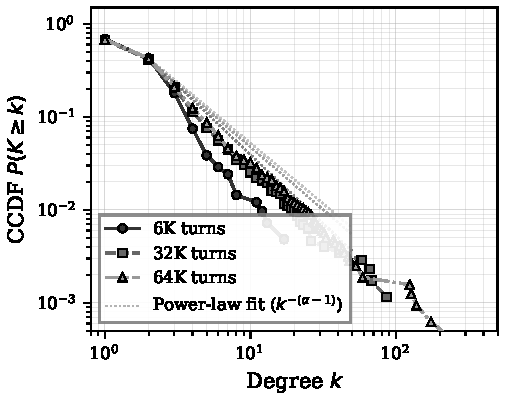
\includegraphics[width=0.85\columnwidth]{figures/fig_degree_distribution.pdf}
\caption{Complementary cumulative degree distribution (CCDF) on log-log axes. Dashed lines: MLE power-law fits. The heavy tail extends with scale.}
\label{fig:degree_dist}
\end{figure}

\paragraph{Graph construction control.}
A natural concern is whether co-occurrence clique construction inflates hub degrees.
We compare against a \textit{typed-relation} graph at 6K that retains only subject$\rightarrow$object edges (no cliques): edge count decreases by 10.4\%, but BFS damage drops only 3.7\% (38.4\% vs 39.8\%).
This confirms that hub degrees are driven primarily by Zipfian entity frequency, not clique construction artifacts.
Extension to 32K/64K remains for future work (see Limitations).

\subsection{Cross-task Contamination}

BFS propagation during FactConsolidation degrades Accurate\_Retrieval F1 by $10.1\pm1.6$pp; \attraware{} preserves accuracy (\cref{app:cross_task}).
This motivates a follow-up question: could hub-concentrated damage be deliberately triggered?


% ============================================================
\section{Hub-Targeted Amplification}
\label{sec:c3}

\subsection{Threat Model}

We evaluate three attacker knowledge levels: \textbf{black-box} (general knowledge), \textbf{gray-box} (hub entity names known), and \textbf{white-box} (fact registry access).
The attacker injects facts through the system's normal memory write interface; conflict detection triggers when a new fact maps to an existing subject-key, initiating the propagation cascade under study.
This write path is realistic: Mem0 and Zep expose memory-write APIs, and MINJA~\citep{minja_2025} demonstrates that even query-only interaction can induce memory writes through indirect prompt injection.
We analyze this vector to inform defensive design; responsible evaluation of adversarial risks is essential for proactive safety.

\subsection{Results}

\begin{table}[htbp]
\centering
\footnotesize
\begin{tabular}{lrrrr}
\toprule
\textbf{Attack} & \textbf{BFS Dam.} & \textbf{BFS Kill} & \textbf{Attr Dam.} \\
\midrule
\multicolumn{4}{l}{\textit{6K Context (344 valid memories)}} \\
1 fact & 5.2\% & 0.3\% & 0.0\% \\
3 facts & 26.7\% & 4.4\% & 0.0\% \\
5 facts & 39.8\% & 17.4\% & 0.3\% \\
\midrule
\multicolumn{4}{l}{\textit{32K Context (1,744 valid memories)}} \\
1 fact & 38.1\% & 1.0\% & 0.0\% \\
5 facts & \textbf{57.3\%} & \textbf{19.3\%} & 1.0\% \\
\bottomrule
\end{tabular}
\caption{White-box adversarial injection at 6K and 32K scales. Kill: weight reduced below retrieval threshold ($< 0.1$). Five facts at 32K damage 57.3\% of valid memories.}
\label{tab:adversarial}
\end{table}

\finding{4} A single fake fact damages 5.2\% (6K) to 38.1\% (32K) of valid memories (\cref{tab:adversarial})---$7.3\times$ amplification from scale and hub-degree growth.
Five facts at 32K degrade 57.3\%, with 19.3\% killed (weight $< 0.1$).

\begin{table}[htbp]
\centering
\footnotesize
\begin{tabular}{lrrr}
\toprule
\textbf{Attack} & \textbf{Facts} & \textbf{Hit} & \textbf{BFS Dam.} \\
\midrule
White-box & 5 & 100\% & 39.8\% \\
Gray-box & 5 & 100\% & 20.9\% \\
Black-box & 5 & 0\% & 0.0\% \\
\bottomrule
\end{tabular}
\caption{Attack comparison at 6K. Black-box fails entirely; gray-box achieves 52\% of white-box damage.}
\label{tab:blackbox}
\end{table}

\finding{5} \Cref{tab:blackbox} shows that under our random-entity black-box baseline, attacks fail to hit hub entities (0\% hit rate).
At minimum, gray-box knowledge of graph structure is needed for the attack vector studied here.
\Cref{fig:depth} shows that damage grows sublinearly with propagation depth while kill rate accelerates due to cumulative decay.

\begin{figure}[ht]
\centering
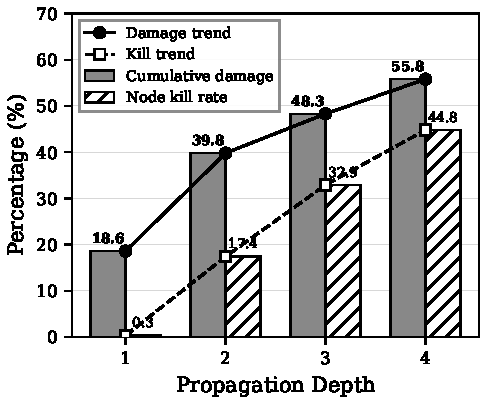
\includegraphics[width=0.85\columnwidth]{figures/fig_propagation_damage.pdf}
\caption{Propagation depth vs collateral damage (6K, 5-fact attack). Damage grows sublinearly while kill rate accelerates due to cumulative decay.}
\label{fig:depth}
\end{figure}


% ============================================================
\section{\attraware{} Selective Propagation}
\label{sec:c4}

\subsection{Method}

The core intuition is directional filtering.
Consider updating ``the CEO of Acme is Alice'' to ``\ldots is Bob.''
In this fact, \textit{Acme} is the subject and \textit{Alice} is the object.
Facts \textit{about Alice} (where Alice is subject)---e.g., ``Alice approves Acme milestones''---may need updating because they depend on Alice's role.
Facts \textit{about Acme} that merely co-occur with Alice---e.g., ``Acme was founded in 2010''---do not, because Acme's founding is independent of who its CEO is.
\attraware{} operationalizes this by following only object$\rightarrow$subject chains: when a fact with subject $s$ and object $o$ is invalidated, propagation continues only to facts where $o$ appears as \textit{subject} (line~4 in \cref{alg:attraware})---restricting cascades to plausible dependency paths:

\begin{algorithm}[htbp]
\caption{\attraware{} Selective Propagation}
\label{alg:attraware}
\begin{algorithmic}[1]
\REQUIRE Invalidated fact $f$ with key $s{:}a$, graph $G$, registry $R$, max depth $D$, decay $\delta$, current depth $h{=}0$
\STATE $s \leftarrow$ subject entity of $f$
\STATE $E_{\text{obj}} \leftarrow$ entities linked to $f$ in $G$, $e \neq s$
\FOR{each $e \in E_{\text{obj}}$}
  \STATE $M_{\text{down}} \leftarrow \{R[k] \mid k.\text{entity} = e\}$ \COMMENT{facts where $e$ is subject}
  \FOR{each $m \in M_{\text{down}}$ if $m$ is valid}
    \STATE $d_{\text{in}} \leftarrow \max(\text{in\_degree}(e, G), 1)$
    \STATE $m.w \leftarrow m.w \times (1 - \frac{1-\delta}{d_{\text{in}}})$
    \IF{$h < D$}
      \STATE \textbf{Propagate}($m, G, R, D, \delta, h{+}1$)
    \ENDIF
  \ENDFOR
\ENDFOR
\end{algorithmic}
\end{algorithm}

The key filtering step is line~4: instead of visiting all graph neighbors, \attraware{} retrieves only facts where the object entity appears as \textit{subject}---restricting propagation to downstream attribute-directed chains.
\attraware{} does not infer causality directly; it uses attribute-keyed directionality as a conservative proxy for dependency.
The in-degree adjustment (line~6) dampens decay for highly-connected entities.
\bfsprop{} differs by visiting all neighbors without semantic filtering or in-degree adjustment.
All operations are string-matching or arithmetic over pre-existing metadata---\textbf{no LLM calls} at propagation time.
At 6K scale (417 nodes, 524 edges), a 5-fact attack completes propagation in $2.3\pm0.2$\,ms for \attraware{} versus $12.8\pm1.2$\,ms for BFS---a $5.5\times$ speedup from reduced traversal scope.
Propagation constitutes $<$5\% of total processing time (dominated by LLM conflict detection), and the full pipeline processes 64K-scale graphs in $<$1\,s without GPU.\footnote{The 64K timing is based on end-to-end pipeline observation; controlled wallclock measurements at 32K/64K scale remain for future work.  The 6K micro-benchmark provides the only formally measured propagation latency.}

\subsection{Propagation Strategy Comparison}

We compare nine propagation strategies spanning structural, weight-based, and semantic filtering approaches (\cref{tab:defense}).

\begin{table}[htbp]
\centering
\scriptsize
\begin{tabular}{lrrrr}
\toprule
\textbf{Strategy} & \textbf{Dam.} & \textbf{Kill} & \textbf{EM} & \textbf{F1} \\
\midrule
\multicolumn{5}{l}{\textit{Unfiltered co-occurrence traversal}} \\
BFS (standard) & 39.8\% & 17.4\% & 10.0\% & 13.3\% \\
BFS + visited set & 39.8\% & 10.2\% & 10.0\% & 13.3\% \\
\midrule
\multicolumn{5}{l}{\textit{Structural constraints}} \\
Degree-cap=5 & 24.1\% & 8.1\% & 10.0\% & 13.3\% \\
Degree-cap=10 & 28.2\% & 10.8\% & 10.0\% & 13.3\% \\
\midrule
\multicolumn{5}{l}{\textit{Threshold-based filtering}} \\
k-hop thresh.\ $\theta{=}0.3$ & 18.6\% & 0.3\% & 20.0\% & 20.0\% \\
k-hop thresh.\ $\theta{=}0.5$ & 18.6\% & 0.3\% & 20.0\% & 20.0\% \\
Weighted BFS $\theta{=}0.1$ & 11.3\% & 3.2\% & 20.0\% & 23.3\% \\
Weighted BFS $\theta{=}0.3$ & 1.5\% & 0.0\% & 20.0\% & 23.3\% \\
\midrule
\multicolumn{5}{l}{\textit{Semantic filtering}} \\
\attraware{} & \textbf{0.3\%} & \textbf{0.0\%} & \textbf{20.0\%} & \textbf{23.3\%} \\
\bottomrule
\end{tabular}
\caption{Propagation strategy comparison (6K, 5-fact white-box attack). Nine strategies spanning unfiltered, structural, threshold-based, and semantic filtering. Weighted BFS ($\theta{=}0.3$) approaches \attraware{} but requires per-deployment threshold tuning; \attraware{} achieves near-zero damage without hyperparameters. EM/F1 are evaluated on 10 adversarial queries; the binary split (10\% vs 20\%) reflects the small evaluation set. Cross-task contamination (\cref{app:cross_task}) confirms $10.1$pp F1 degradation on a larger evaluation set.}
\label{tab:defense}
\end{table}

\finding{6} \Cref{tab:defense} reveals a spectrum from structural constraints (degree capping, modest reduction) through threshold-based filters (weighted BFS at $\theta{=}0.3$: 1.5\% damage) to semantic filtering (\attraware{}: 0.3\%).
Threshold methods require per-deployment tuning and exhibit cliff effects (k-hop $\theta{=}0.3$ and $0.5$ produce identical results); \attraware{} requires no hyperparameters.
At 32K/64K scale, Weighted BFS $\theta{=}0.3$ maintains 0.2\%/0.1\% damage---comparable to \attraware{}'s 1.0\%/0.9\%---while BFS standard damage escalates to 57.3\%/61.6\% (from 39.8\% at 6K).
Both filtered strategies remain effective even as hub degrees grow to 298; the practical advantage of \attraware{} lies in hyperparameter-free operation, avoiding the cliff effects and per-deployment $\theta$-tuning that threshold methods require.

\subsection{Cross-experiment Consistency}

\begin{table}[htbp]
\centering
\footnotesize
\begin{tabular}{lrrrr}
\toprule
\textbf{Experiment} & \textbf{BFS} & \textbf{WBFS} & \textbf{Attr} & \textbf{Def.} \\
\midrule
Scale 6K--64K & 69--79\% & --- & 15\% & 78--81\% \\
Cross-task (F1) & $-$10.1pp & --- & +0.0pp & 100\% \\
Adv 6K / 5f & 39.8\% & 1.5\% & 0.3\% & 99.3\% \\
Adv 32K / 5f & 57.3\% & 0.2\% & 1.0\% & 98.2\% \\
Adv 64K / 5f & 61.6\% & 0.1\% & 0.9\% & 98.5\% \\
\bottomrule
\end{tabular}
\caption{Defense effectiveness across all experiments. \textbf{Def.} = $1 - \text{Attr}/\text{BFS}$. WBFS = Weighted BFS $\theta{=}0.3$ (best per-scale). At 32K/64K, WBFS achieves lower absolute damage than \attraware{}, but requires per-deployment $\theta$-tuning. Cross-task: BFS degrades F1 by $10.1\pm1.6$pp; \attraware{} preserves accuracy.}
\label{tab:defense_all}
\end{table}

\finding{7} \Cref{tab:defense_all} shows that \attraware{} achieves 78--100\% defense effectiveness (measured as $1 - \text{Attr}/\text{BFS}$, i.e., relative to unfiltered BFS, not vs.\ best available alternative) across all experimental conditions.
The strongest evidence comes from cross-task contamination, where \attraware{} fully preserves retrieval accuracy ($\Delta$F1 = 0.0pp) against BFS's $-$10.1pp degradation---evaluated on a larger query set than the adversarial EM/F1 comparison (which uses only 10 queries and produces binary splits).

\subsection{Robustness to BFS Variants}

A natural concern is whether BFS damage is inflated by redundant decay (a node decayed multiple times via different paths) or a particular decay parameter.
We test variants at both 6K and 32K under the 5-fact white-box attack (\cref{tab:robust}).

\begin{table}[htbp]
\centering
\scriptsize
\begin{tabular}{llrrrr}
\toprule
\textbf{Scale} & \textbf{BFS Variant} & \textbf{Dam.} & \textbf{Sev.} & \textbf{Kill} \\
\midrule
\multirow{5}{*}{6K} & Standard (decay=0.5) & 39.8\% & 11.1\% & 17.4\% \\
& + memory visited set & 39.8\% & --- & 10.5\% \\
\cmidrule{2-5}
& decay = 0.3 & 39.8\% & 11.9\% & 20.1\% \\
& decay = 0.7 & 39.8\% & 19.8\% & 2.0\% \\
& decay = 0.9 & 39.8\% & 2.0\% & 0.0\% \\
\midrule
\multirow{2}{*}{32K} & Standard (decay=0.5) & 57.3\% & --- & 19.3\% \\
& + memory visited set & 57.3\% & --- & 7.8\% \\
\bottomrule
\end{tabular}
\caption{BFS damage is structurally determined: damage rate is identical across all variants within each scale (39.8\% at 6K, 57.3\% at 32K). Sev.\ = severe damage ($0.1 \leq w < 0.5$). At the default decay=0.5, 28.5\% of valid memories suffer kill or severe damage.}
\label{tab:robust}
\end{table}

\finding{8} \Cref{tab:robust} reveals that damage rate is invariant to both redundant-decay elimination and decay parameter choice at \textit{both} scales.
The 39.8\% (6K) and 57.3\% (32K) damage rates reflect BFS \textit{reachability}---the fraction of memories structurally connected to hub entities within depth~2---not an artifact of parameter tuning or implementation choices.
At the default decay of~0.5, 28.5\% of valid memories suffer severe or lethal weight reduction ($w < 0.5$), confirming that damage is not merely cosmetic.
Even at decay=0.9 (the most conservative setting), 2.0\% of memories are severely damaged despite zero kills---and the 39.8\% damage rate persists.
The higher 32K rate confirms that structural vulnerability increases with scale as hub degree grows ($23 \rightarrow 121$).


% ============================================================
\section{Related Work}
\label{sec:related}

\paragraph{Memory invalidation and belief revision.}
Kumiho~\citep{kumiho_2026} maps AGM belief revision postulates~\citep{agm_1985} to a property graph with typed dependency edges, providing formal guarantees that unrelated beliefs are preserved.
Our work is complementary: Kumiho shows \textit{why} typed edges are needed (axiomatic); we show \textit{what happens without them} (empirical), providing the damage quantification that motivates architectural choices like Kumiho's.
MaRS~\citep{mars_2025} compares six forgetting policies with provenance closure constraints on the retention side; our study addresses the invalidation side.

\paragraph{Memory security.}
MINJA~\citep{minja_2025}, AgentPoison~\citep{agentpoison_2024}, and ER-MIA~\citep{ermia_2026} inject malicious content.
KEPo~\citep{kepo_2026} and LogicPoison~\citep{logicpoison_2026} manipulate graph topology.
Our attack is structurally distinct: it triggers the system's own forgetting mechanism rather than injecting content or manipulating retrieval paths.

\paragraph{Network resilience.}
Heavy-tailed networks exhibit robust-yet-fragile behavior under targeted hub removal~\citep{albert_attack_2000, cohen_percolation_2000}.
Our results are consistent with this pattern in AI memory graphs ($\alpha \approx 2.7$--$3.0$, heavy-tailed).


% ============================================================
\section{Discussion and Conclusion}
\label{sec:conclusion}

\paragraph{Key message.}
Our stress-test evaluation identifies \textbf{memory graph propagation} as a design choice that demands caution.
Unfiltered co-occurrence traversal produces collateral damage (69--79\%), enables low-cost adversarial amplification (5 facts $\rightarrow$ 57.3\% degradation), and contaminates unrelated tasks (F1 $-$10.1pp).
Both \attraware{} and tuned threshold filtering (Weighted BFS $\theta{=}0.3$) reduce these risks by $\geq$98\% at scale---demonstrating that dependency-aware propagation is both necessary and achievable.
\attraware{}'s advantage is hyperparameter-free operation; Weighted BFS achieves lower absolute damage at 32K/64K but requires per-deployment $\theta$-selection and is vulnerable to cliff effects. The optimal filtering strategy remains an open problem.

In the co-occurrence graph setting evaluated here, our results support a design principle: \textbf{propagation should incorporate dependency awareness rather than relying on raw structural co-occurrence}.
This insight is well-established in transportation network resilience; we demonstrate its relevance to AI memory systems built on entity co-occurrence graphs.
By characterizing these failure modes before any production system adopts unfiltered graph-based propagation, this work serves as proactive safety research---identifying risks while mitigation is still a design choice rather than a retrofit.

\paragraph{Implications for memory system design.}
Systems adopting unfiltered propagation over untyped co-occurrence graphs are vulnerable to hub-amplified damage.
The attack is low-cost (5 facts), scales with memory size, and operates through legitimate maintenance pathways.
Hub entities cannot be removed as they are essential for retrieval; \attraware{} functions as a \textit{safety guardrail}, constraining propagation---including learned policies~\citep{mars_2025}---to plausible dependency chains.

\paragraph{Generalizability.}
Entity mention frequencies follow Zipf's law~\citep{zipf_1949}, producing hub-and-spoke structures in co-occurrence graphs regardless of domain~\citep{steyvers_semantic_2005, barabasi_scalefree_1999}.
While replication on additional benchmarks is important, the Zipfian origin of hub formation suggests our results generalize beyond MemoryAgentBench.

\paragraph{Limitations.}
(1) Single benchmark (MemoryAgentBench); the Zipfian argument above is theoretical, not empirical.
(2) Single LLM (Gemma-4-31B-it); while entity extraction is rule-based and graph topology drives core findings, LLM-dependent conflict detection may behave differently across model families---replication with diverse LLMs is an important next step.
(3) Under the 5-fact adversarial attack (\cref{tab:adversarial}), \attraware{} damaged only 6 memories at 6K (5 directly invalidated targets + 1 propagation-damaged); manual inspection of all~6 confirmed the single propagation case as legitimate cascade (zero false positives).
Separately, the ${\sim}$15\% organic damage in \cref{tab:scale} (${\sim}$51 memories at 6K) arises from natural conflicts during memorization.
Full classification of all~51 organic-damaged memories (single annotator; criterion: whether an explicit subject$\rightarrow$object dependency chain exists between the invalidated and damaged facts) found \textbf{88.2\% legitimate cascade}, \textbf{11.8\% borderline} (graph-connected, dependency uncertain), and \textbf{zero false positives}.
The 32K/64K organic residual awaits similar full classification.
(4) Propagation depth is fixed at 2; decay sensitivity analysis (\cref{tab:robust}) shows damage rate is structurally invariant to decay but kill rate varies---full depth$\times$decay sweeps remain for future work.
(5) Co-occurrence clique construction may amplify hub degrees; our typed-relation control (\cref{sec:c1}) shows only modest impact at 6K, but extension to 32K/64K remains for future work.
(6) No current deployed memory system implements the BFS invalidation policy evaluated here; we evaluate a natural design extension that existing graph prerequisites make straightforward to adopt, as evidenced by community requests for consistency propagation in production systems.\footnote{See Introduction footnote for specific examples.}
(7) The BFS implementation does not maintain a memory-level visited set; however, \cref{tab:robust} shows that adding one does not change damage rate (only kill rate decreases by 6.9pp), confirming that damage is driven by structural reachability rather than redundant decay.

\paragraph{Future work.}
(1) Extend the typed-relation graph comparison (Limitation~5) to 32K/64K scales and evaluate \attraware{} on typed graphs.
(2) Validate on production memory systems (Mem0$^g$, Zep) once they implement propagation.
(3) Although our experiments use text-derived fact graphs, the underlying issue is not text-specific.
Multimodal agents maintain episodic, semantic, and visual memories sharing entity references, and the co-occurrence-versus-dependency distinction applies when cross-modal updates should or should not cascade.

% ============================================================
\section*{LLM/Agent Usage Disclosure}

This research used LLM-based tools in three capacities:
(1)~Literature search and survey assistance (paper discovery and classification);
(2)~LaTeX editing and proofreading;
(3)~Experimental code development (benchmark integration, graph analysis scripts).
All experimental results, analysis, and conclusions were produced and validated by the authors.
The core experimental pipeline (entity extraction, subject-key matching, propagation algorithms) uses rule-based methods without LLM involvement at runtime, except for conflict detection which uses Gemma-4-31B-it as specified in the experimental setup.


% ============================================================
\bibliography{references}
\bibliographystyle{icml2026}


% ============================================================
\appendix

\section{Cross-task Contamination (C2)}
\label{app:cross_task}

BFS propagation from a single hub entity (``Debbie'', degree=715 in the EventQA graph) cascades to 3,381 memories, causing EM $-5.0$pp and F1 $-18.2$pp on completely unrelated retrieval queries.
Across the top-5 hubs, BFS consistently degrades F1 by $10.1\pm1.6$pp.
\attraware{} preserves full accuracy (F1 $71.1\pm1.3$\% vs baseline $70.9$\%).

\section{Multi-run Statistics}
\label{app:stats}

We run the 6K adversarial attack 7 times (19 paired observations).
Pooled Wilcoxon signed-rank test: $W = 86.0$, $p = 0.0022$; bootstrap 95\% BCa CI $[2.82, 15.67]$pp excludes zero.
A mixed-effects model with attack strength as fixed effect and run as random intercept confirms the 5-fact condition is significant ($p = 0.020$).

\section{Graph Construction}
\label{app:graph}

Entity extraction uses rule-based proper noun detection and ``the X of Y'' patterns.
Co-occurrence edges form cliques per fact.
Subject-keys are deterministic: ``the president of Russia is Putin'' $\rightarrow$ \texttt{Russia:president}.
Conflict is triggered when a new fact maps to an existing subject-key.

\section{Experimental Configuration}
\label{app:config}

LLM: Gemma-4-31B-it (temp=0.0). Embedding: BAAI/bge-m3 (1024-dim). Graph: NetworkX DiGraph. Storage: SQLite in-memory. Benchmark: MemoryAgentBench (ICLR 2026). Scales: 6K/32K/64K. Propagation: depth=2, decay=0.5.


\end{document}
